
\chapter{Introduction}

With increasing cases of atrocities on women and children during their commute, there is a need for an advanced system to quickly notify police in case of emergency. Most of the cases remain a mystery due to lack of evidence. We propose a system that help the victims to send a distress signal to police by pressing an emergency button or by activating it with their voice.
 
%This chapter introduces the product to the reader and is called the
%\emph{product brief}. It contains the following sections. The questions
%raised in the following sections are representative of a generic product.
%These questions need to be addressed through the contents written
%in this chapter. It should be noted that the questions are not exhaustive.
%If however, you feel that the questions do not address a specific
%need for your product, then do not hesitate to address them too.


\section{Background}

The crime against women as reported by National Crime Record Bureau of India (NCRBI), has increased by 9.9\% in 2014. Around 3,25,329 crimes against women were reported in India in 2014, which includes rape, kidnapping and abduction of women, dowry deaths, assault on women with intent to outrage her modesty, insult to the modesty of women, cruelty by husband or his relatives etc.

A total of 57,311 cases were reported under kidnapping and abduction of women during 2014. These cases have shown an increase of 10.5\% during 2014 over the year 2013. Figure~\ref{fig:pie} summarizes the NCRBI report\cite{ncrbi} on crimes against women.

\begin{figure}[H]
\centering
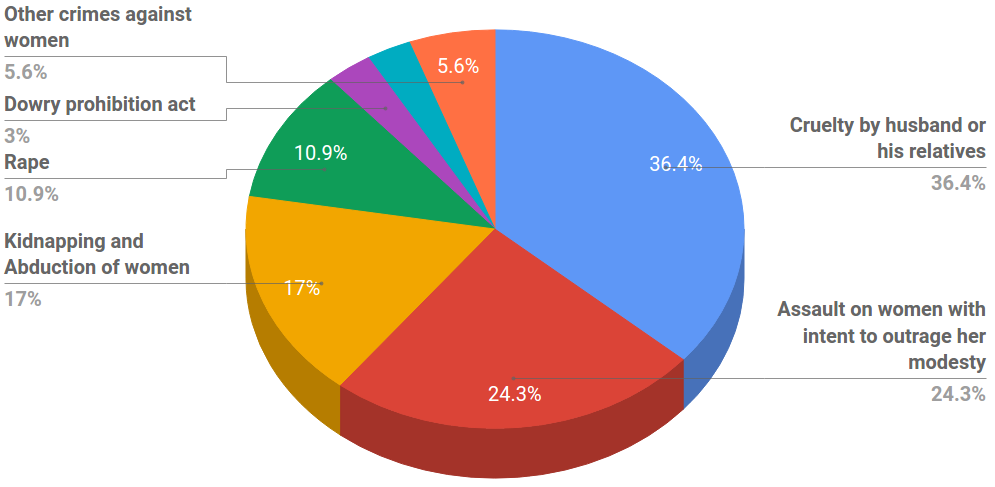
\includegraphics[width=\textwidth]{pie}
\caption{Chart for recorded number of crime against women}
\label{fig:pie}
\end{figure}

Many of these happen in public transport vehicles like buses and cabs. Hence the government (Ministry of Highways and Road Transport) has recently issued a circular mandating a connected panic button which can be pressed by the victim in case of a distress situation. The button will send an SOS to the nearest Police Control Room (PCR) for prompt action. Next  section describes the functional requirements of such device in detail.
%In the following section, we present an abstract view of the functions performed by this device, in order to reduce the number of crime against women. 
%Give the motivation and need with figures and block diagrams to explain
%your project.


\section{Functional aspects}
Our idea is to install \emph{PanicButton device} in all public transport vehicles. It triggers an emergency, if either panic button is pressed or scream is detected. Audio-based trigger monitors the surrounding in the real time and asserts an emergency in case of scream detection. The \emph{PanicButton device} conveys the message of emergency to the back-end server over a wireless link.
Figure~\ref{fig:safecommute} shows the proceedings of a safe commute with our device installed in it.

The following secondary functions are also performed by the \emph{PanicButton device}-
\begin{itemize}
\item self-check,
\item indicate the status using back-light installed in emergency button,
\item providing realtime vehicle location updates,  
\item providing panic button validation service and,
\item providing driver and vehicle details to the user.
\end{itemize}

\begin{figure}[H]
\centering
\def\svgwidth{\textwidth}
\input{safecommute.pdf_tex}
\caption{A safe ride with our device in vehicles}
\label{fig:safecommute}
\end{figure}
 
%The following questions need to be addressed:
%\begin{itemize}
%\item What is the primary function of the proposed product?
%\item What are the secondary functions if any?
%\item Does a similar product exsit in the market?
%\item Does the product form a part of a bigger system or should it work
%in conjuction with other equipments?
%\item Are there any standards or protocols that need to be followed?
%\end{itemize}

%\section{User aspects}

%The following questions need to be addressed:
%\begin{itemize}
%\item What is the technical competence of the user?
%\item Is there any constant user-product interaction required?
%\item What are the ergonomical constraints brought in by the usage pattern?
%\item Is the product operated continuously or intermittently?
%\item What will be the specific documentation of the product that is required
%by the user?
%\item Is the user required to perform installation and maintenance?
%\end{itemize}

\section{User interfaces and communication channels}
User can interact with the \emph{PanicButton device} in following ways.
\begin{itemize}
\item using the panic button,
\item using microphone available on the device and,
\item using the dedicated android application.
\end{itemize}
Panic button is designed to be easily accessible; this was ensured by its large size and always-on back-light. Physically disabled and immobilized victims can use the internal microphone to interact with the \emph{PanicButton device}. Audio-based trigger takes input from this microphone and scan the audio stream for screams. Emergency is asserted in case a scream is detected. User can interact with the \emph{PanicButton device} for its validation using the dedicated android application.

The \emph{PanicButton device} requires four communication channels in order to work at it's full potential.
%We need four communication channels to take full benefit of the service.
\begin{itemize}
\item Wireless communication channel between the \emph{PanicButton device} and the back-end server,
\item Wireless communication channel between the \emph{PanicButton device} and the user's smartphone,
\item Internet link between the user's smartphone and the back-end server.
\item Internet link between the back-end server and PCRs.
\end{itemize}

%\section{Characteristics and performance}

%The following questions need to be addressed:
%\begin{itemize}
%\item What are the parameters to be measured, monitored and controlled by
%the product or product system?
%\item What are the performance requirements that is expected of the product?
%\item Are there any absolute maximum ratings on any of the input or output
%parameters?
%\item Which are the variables that are likely to influence the performance
%of the product?
%\item Are there any special considerations about the input and/or output
%signals?
%\end{itemize}

%\section{Environment aspects}

%The following questions need to be addressed:
%\begin{itemize}
%\item How do you classify the application of the product from the environmental
%point of view? (\emph{Refer to MIL-STD for environmental classifications
%on the web})
%\item What is the ambient temperature range in the neighbourhood of the
%product?
%\item Do humidity, vibration and pressure affect the operation and design
%of the product?
%\item What other environmental parameters have significant impact on the
%product operation?
%\end{itemize}

\section{Power supply}
Vehicle's battery is the primary power supply for the \emph{PanicButton device}. The primary power supply also charges a secondary battery, which resides inside the \emph{PanicButton device}. In case of breakdown in primary power supply, secondary battery can power the \emph{PanicButton device} for couple of hours. In case of breakdown of both primary and secondary sources of power, an ultra low power circuitry powered by an independent source, takes the note of event and informs the back-end server on power restoration. Over all we have two power sources for complete system and an independent power source for an ultra low power system monitoring circuit.


%The following questions need to be addressed:
%\begin{itemize}
%\item Is the product battery operated?
%\item What will be the effect of a power breakdown on the product or the
%associated system?
%\item Are there special considerations or limitations on the power consumption
%of the product?
%\end{itemize}

%\section{Safety}

%The following questions need to be addressed:
%\begin{itemize}
%\item In case of supply voltages upto 270V with respect to earth, what is
%the nature of the location in which the equipment is to be installed?
%\item What is the class of the product from the point of view of the safety
%standards? (\emph{refer to web})
%\end{itemize}

%\section{Reliability}

%The following questions need to be addressed:
%\begin{itemize}
%\item What is the warranty/gaurantee conditions that will be proposed for
%your product?
%\item What is the targeted reliability figure in terms of MTTF(mean time
%to failure)?
%\item What is the proposed service infrastructure for the product?
%\item What should be the operational downtime to uptime ratio for the product?
%\item What is the targeted maintainability figure in terms of MTTR(mean
%time to repair)?
%\end{itemize}

%\section{Literature Survey}

%The following questions need to be addressed:
%\begin{itemize}
%\item What is the existing status of technology or algorithms in relation
%to the product/project?
%\item What are the gaps the proposed product/project addresses?
%\end{itemize}

\section{Product/market Survey}
Most of the safety device market is clustered towards the private safety services. Our \emph{PanicButton device} provides public safety service for people, who uses public transport vehicle. Devices serving this purpose are yet to make impact in the safety-service market.

Wearable safety devices occupies major chunk of safety-service market. These devices uses smartphone as relay between the user and their guardians. These devices come in  the form of a wrist band, a pendant, a necklace and an earrings. They all have small form factor and a constrained power supply. Generally these devices rely on paired smartphone in its vicinity for long-range communication. Wearables device communicates with the smartphone over low energy short range links mainly Bluetooth low enregy (BLE). Some wearable safety devices comes with a microphone to record audio as evidences. Some of the popular brands in this category are Artemis, Amulyte, Stiletto, Cuff, Safer, Revolar and First sign. Table~\ref{tab:markettable} summarizes their characteristics.
\begin{table}[H]
\begin{center}
\begin{tabular}{ |c|c|c|c| } 
 \hline
 \textbf{Brand} & \textbf{Trigger} & \textbf{Audio support} &\textbf{Standalone}\\
 \hline 
 Artemis(pendent,clips)\cite{safe1} & 3 Button presses & Microphone & No \\
\hline 
Amulyte(pendent)\cite{safe2} & Button press & Microphone \& speaker & No \\
\hline
Stiletto(pendent)\cite{safe3} & Button press & Microphone \& speaker & No \\
\hline
CUFF (pendent)\cite{safe4} & Button press & No & No \\
\hline
SAFER (pendent)\cite{safe5} & 2 Button presses & No & No \\
\hline
Revolar (clip)\cite{safe6} & Button press & No & No \\
\hline 
Fisrt sign (watch)\cite{safe7} & 2 Button presses & No & No \\
 \hline
\end{tabular}
\end{center}
\caption{Characteristics of a few well known safety wearables in the safety-service market} 
\label{tab:markettable}
\end{table}

The \emph{PanicButton device} is a complete standalone package with all the necessary hardware and software packed in a 6"x6"x2" box.
%The following questions need to be addressed:
%\begin{itemize}
%\item Are there similar products in the market?
%\item What are its \emph{features}? (Prepare a comparison table of \emph{features}
%in relation to the proposed product/project)
%\end{itemize}

%\section{User Survey}

%The following questions need to be addressed:
%\begin{itemize}
%\item Who are the users of the product?
%\item Are the users technical or non-technical people?
%\item What are their opinions on the features of the proposed product?
%\item What are the features that are desirable in their opinion, but are
%not possible to implement in your opinion?
%\end{itemize}

\section{Wish scope}
Wish scope is to capture each and every distress moments in the vehicle and trigger an emergency alarm. Make the \emph{PanicButton device} tamper-proof and have ubiquitous connectivity with all required devices. In the next chapter we take a look at available technology/algorithms and give a realistic scope.
%The following questions need to be addressed:
%\begin{itemize}
%\item What is the scope of the product that you wish to undertake?
%\item What is the set of dream/wish specifications that you consider would
%be ideal for your product?
%\item Prepare a comparison table of the specifications of similar existing
%products in relation to the proposed product/project\end{itemize}
